\chapter{Problem Introduction}
\label{chap:problem-introduction}

\section{Problem Statement}
Learning Vietnamese Sign Language (VSL) remains a challenge because existing learning resources are often fragmented across videos, social media posts, classroom notes, and small independent websites. In practice, learners usually do not have access to a centralized platform where they can search vocabulary, follow structured learning paths, enroll in courses, monitor their progress, and maintain long-term motivation. This also creates difficulties for teachers and administrators who need to manage educational content and learner activity in a consistent and systematic way.

The educational problem is therefore not only about delivering content, but also about organizing learning data in a way that supports real teaching and learning workflows. A dedicated online platform for Vietnamese sign language requires an integrated database capable of handling users, roles, vocabulary resources, courses, lessons, enrollments, progress records, feedback, notifications, and learner engagement data. Without such a database foundation, the platform would face problems of redundancy, inconsistency, and poor maintainability.

To address this need, the project develops a database system for an online Vietnamese sign language learning platform. The system is intended not only to store information, but also to support practical educational processes such as student enrollment, progress updates, streak tracking, notifications, reporting, and interaction through a database demo application.

\begin{figure}[htbp]
    \centering
    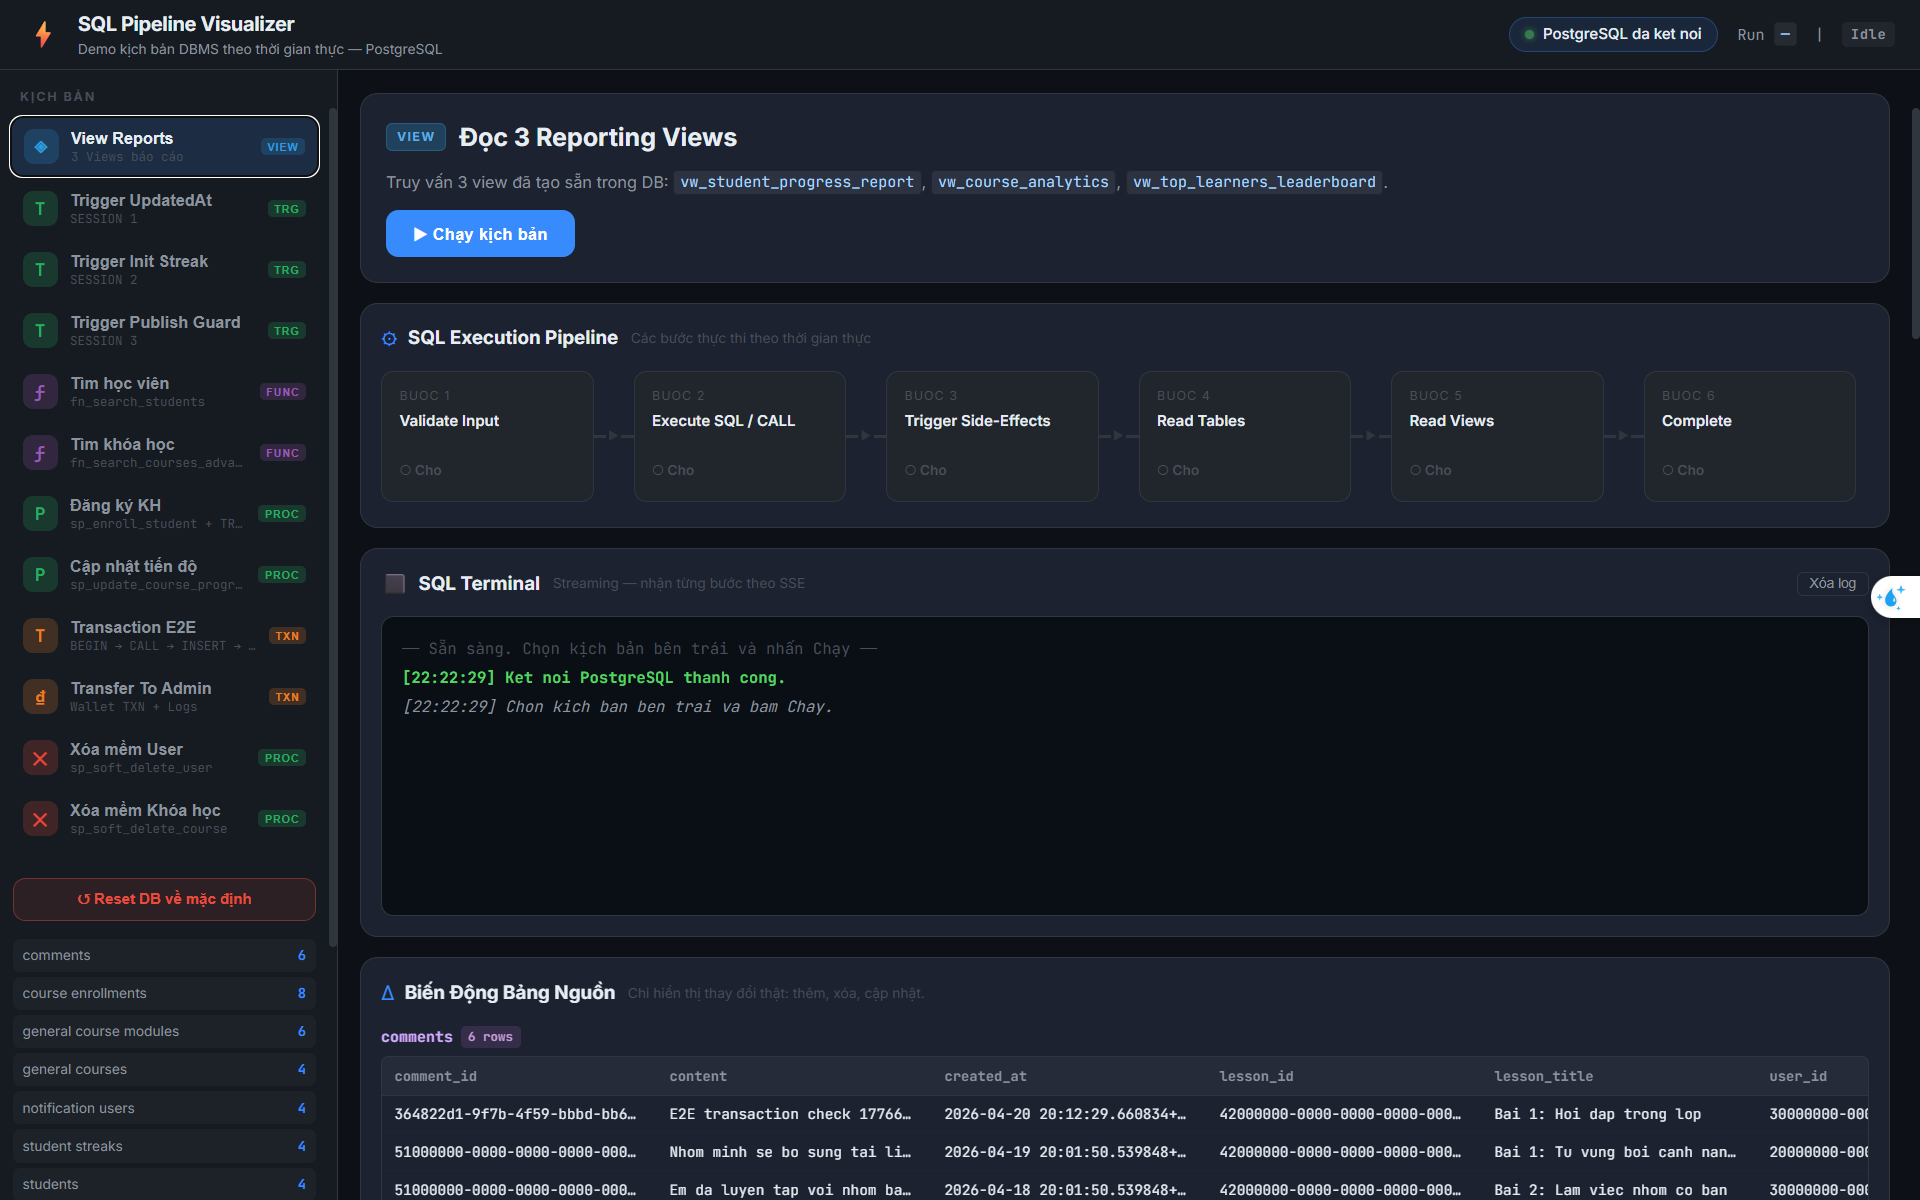
\includegraphics[width=0.9\textwidth]{assets/images/figure_1_1}
    \caption{Problem context and motivation for building the Vietnamese sign language learning platform.}
    \label{fig:introduction-context}
\end{figure}

\section{Project Objectives}
The main objective of this project is to design and implement a reliable database foundation for an online Vietnamese sign language learning platform. The database must support the storage, retrieval, and controlled processing of information related to learners, teachers, courses, lessons, dictionary content, and learning activities.

From a database perspective, the project is expected to organize data clearly, maintain consistency, support access control, and provide a stable basis for learning-related operations. More specifically, the project aims to:
\begin{itemize}
    \item design a normalized relational schema that clearly represents the key entities and relationships of the system;
    \item ensure data consistency through primary keys, foreign keys, unique constraints, check constraints, and transaction control;
    \item implement database-side business logic using views, functions, procedures, and triggers;
    \item support role-based access patterns for administrators, teachers, and students;
    \item provide data structures for enrollments, progress tracking, comments, notifications, and engagement features;
    \item prepare the database for integration with a web-based demo application that illustrates major workflows.
\end{itemize}

\section{Scope and Limitations}
The scope of the project focuses on the database layer of the platform. It includes the design and implementation of modules for user management, authentication sessions, sign language dictionary content, course organization, lesson materials, student enrollments, learning progress, comments, microlearning, gamification, notifications, and transaction logging. The project also covers database mechanisms such as views, functions, procedures, triggers, soft delete, and transaction handling for important business scenarios.

However, the current implementation also has clear limitations. First, the project focuses mainly on database design and backend processing rather than full-scale production deployment. Second, advanced multimedia and intelligent features such as sign recognition, automatic interpretation, or AI-based translation are outside the current scope. Third, performance benchmarking, large-scale concurrency testing, and production-grade infrastructure evaluation are limited, because the project is mainly intended for academic demonstration and database system practice.

\begin{figure}[htbp]
    \centering
    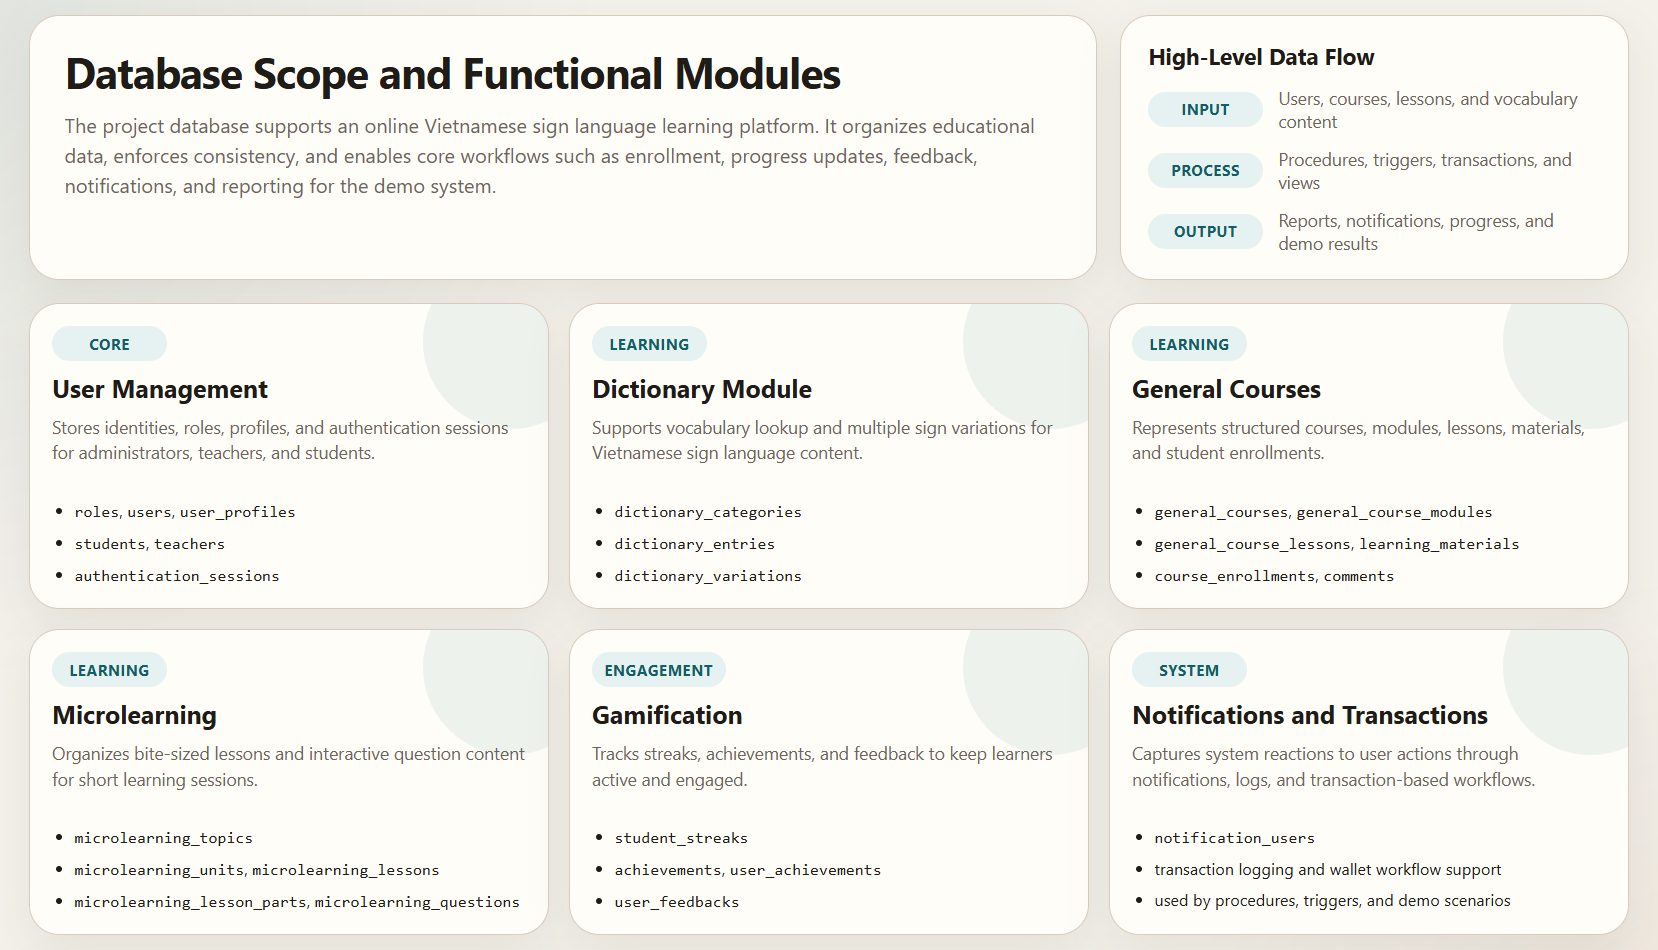
\includegraphics[width=0.9\textwidth]{assets/images/figure_1_2}
    \caption{Scope of the database system and major functional modules.}
    \label{fig:introduction-overview}
\end{figure}

\section{Report Structure}
This report is organized into several chapters that follow the development process of the project. Chapter~1 introduces the problem context, project objectives, scope, limitations, and general motivation of the study. Chapter~2 presents the configuration process, tools, technologies, and platforms used during development. Chapter~3 focuses on database design, including the entity--relationship model, schema organization, constraints, and relationships among the main modules. Chapter~4 explains the implementation details of the database system, especially the use of views, functions, procedures, triggers, and transactions, together with the demo workflow. Chapter~5 concludes the report by summarizing the main results, limitations, and possible future improvements. In addition, the report also includes a references section and appendices for supporting technical materials such as SQL scripts.
